%!TEX root = Slic3r-Manual.tex

\section{Calcul des flux} % (fold)
\label{sec:flow_math}
\index{flow math}
\index{Calcul des flux}

Cette page explique les calculs utilis\'ees dans Slic3r pour d\'eterminer la quantit\'e de flux. La documentation sert de r\'ef\'erence, car il pourrait être utile d'essayer de meilleurs mod\`eles.

\subsection{Comprendre la largeur d'extrusion} % (fold)

Deux questions principales affectent le travail de Slic3r:
\begin{itemize}
\item \textbf{A quelle distance} les chemins d'extrusion doivent-ils être positionn\'es pour obtenir une finition r\'eguli\`ere?
\item \textbf{Quelle quantit\'e de mati\`ere} doit être extrud\'ee le long de ces chemins?
\end{itemize}

Si deux chemins adjacents sont \textbf{trop proches} (ou \textbf{trop de mati\`ere} est extrud\'ee), ils se chevauchent. Si deux chemins adjacents sont \textbf{trop \'eloign\'es} (ou si \textbf{le mat\'eriau est insuffisamment extrud\'e}), des interstices seront visibles et / ou les extrusions se d\'etacheront en raison d'une liaison insuffisante.

En extrudant plus ou moins tout en se d\'eplaçant (c'est-\`a-dire en changeant \textbf{le rapport vitesse de flux/vitesse tête}), on peut faire des chemins plus \'epais ou plus minces:

\begin{figure}[H]
\centering
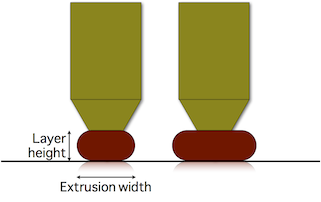
\includegraphics[keepaspectratio=true,width=0.5\textwidth]{advanced/flow_math/extrusion_width.png}
\caption{Largeur d'extrusion}
\label{fig:extrusion_width}
\end{figure}

\textbf{Des chemins plus \'epais} auront \textbf{une meilleure liaison} avec la couche inf\'erieure, ce qui est bon pour les pi\`eces m\'ecaniques. Cependant, ils seront moins en mesure de rapprocher la forme de l'objet et de combler de minuscules lacunes ou des courbes \'etroites (pensez \`a un foret: un plus grand ne sera pas en mesure d'entrer dans des endroits \'etroits). Au contraire, \textbf{des chemins plus minces} fourniront moins de collage mais une meilleure pr\'ecision de forme.

Noter cependant que la largeur d'extrusion ne peut être contrôl\'ee que lors de l'extrusion sur une surface existante (telle qu'une couche pr\'ec\'edente ou un lit d'impression). Si on extrude \texttt{\`a l'air libre} (c'est-\`a-dire en pontage), la forme r\'esultante sera toujours \textbf{ronde} et \'egale au \textbf{diam\`etre de la buse}:

\begin{figure}[H]
\centering

\includegraphics[keepaspectratio=true,width=0.5\textwidth]{advanced/flow_math/bridge.png}
\caption{Section d'un pont}
\label{fig:bridge}
\end{figure}

En fait, si vous r\'eduisez le flux de mati\`ere, vous obtiendrez des cercles plus petits dans une certaine mesure, jusqu'\`a ce que la viscosit\'e plastique d\'ecide qu'il est temps de briser votre pont en raison de trop de tension. Si, au contraire, vous extrudez trop de mat\'eriau, la forme du filament extrud\'e ne changera pas (toujours \'egale au diam\`etre de la buse), mais vous obtiendrez un pont distandu.

Alors, partons d'une d\'efinition:

La largeur d'extrusion est \textbf{l'\'epaisseur d'un seul filament} extrud\'e soit \`a l'air libre, soit au-dessus d'une surface. Ce n'est \textbf{pas} la distance de deux chemins adjacents car un chevauchement sera g\'en\'eralement appliqu\'e afin d'obtenir une meilleure liaison.

\subsection{Ponts: le cas facile} % (fold)

Comme indiqu\'e ci-dessus, il n'y a qu'un seul d\'ebit correct pour le pontage: celui qui ne fait pas que votre pont s'affaisse ou se casse. Les extrusions sont \textbf{rondes} et leur \textbf{diam\`etre est \'egal au diam\`etre de la buse}. Des trajets parall\`eles seront positionn\'es de telle sorte qu'ils soient \textbf{tangents}, ainsi l'espacement entre un chemin et son voisin est \'egal au diam\`etre de la buse aussi. (Dans le cas des ponts, nous ne voulons pas de chevauchement car il a prouv\'e de tra\^iner les chemins existants.)

Le volume de mati\`ere requis pour un trajet de longueur unitaire est calcul\'e en cons\'equence \`a la forme cylindrique, donc avec une section transversale circulaire:

$E = (diametre buse/2)^2 * pi$

\subsection{Extrusion sur une surface} % (fold)

Dans ce cas le probl\`eme est: \texttt{quelle forme} notre extrusion obtenir? Nous savons qu'il sera \'ecras\'e horizontalement, mais aura-t-il une forme rectangulaire ou ovale? Quelle est la largeur d'extrusion maximale que nous pouvons obtenir avec un diam\`etre de buse donn\'e avant que le plastique commence \`a se recourber sur les côt\'es?

Slic3r suppose que la forme en coupe transversale d'une extrusion est un rectangle \`a extr\'emit\'es semi-circulaires. Ainsi, la relation entre la largeur et le volume d'extrusion souhait\'es pour extruder est la suivante:

\begin{figure}[H]
\centering
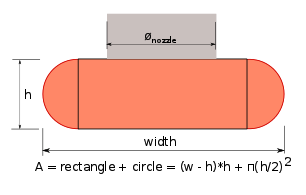
\includegraphics[keepaspectratio=true,width=0.5\textwidth]{advanced/flow_math/area1.png}
\caption{coupe transversale de l'extrusion}
\label{fig:area1}
\end{figure}

Lorsque la largeur d'extrusion de la cible est plus fine que la hauteur de la couche, la forme est impr\'evisible, nous utilisons simplement la même formule rectangulaire mais d\'ecourager l'utilisation de telles valeurs d'extrusion minces.

La formule ci-dessus fournit une fonction qui corr\`ele la largeur d'extrusion cible avec la quantit\'e de mati\`ere \`a extruder par unit\'e de distance:

$E = f(largeur extrusion, hauteur couche)$

\subsection{Espacement des passage} % (fold)

Bon, maintenant nous savons combien extruder pour faire un seul chemin de la largeur d\'esir\'ee. Mais \textbf{\`a quel point devrions-nous chevaucher} des chemins afin d'obtenir une liaison parfaite?

En supposant qu'il n'y ait pas de chevauchement, donc de trajectoires tangentes, il y aurait un espace vide (jaune):

\begin{figure}[H]
\centering
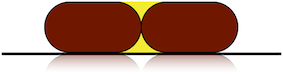
\includegraphics[keepaspectratio=true,width=0.5\textwidth]{advanced/flow_math/tangent.png}
\caption{coupe transversale de l'extrusion}
\label{fig:tangent}
\end{figure}

La section transversale de ces vides est g\'en\'eralement:

$aire vide = hauteur couche^2 - (hauteur couche/2)^2 * pi$

Id\'ealement, nous voudrions remplir toute cette zone jaune en plaçant les extrusions ferm\'ees les unes aux autres. Cependant, il est tr\`es peu probable que la seconde extrusion remplisse l'espace sous la pr\'ec\'edente, il y aurait donc un peu de vide. Le chevauchement id\'eal serait quelque chose comme:


$0 < facteur de recouvrement*aire vide < aire vide$


Avec \texttt{facteur de recouvrement} allant de 0 \`a 1. \texttt{facteur de recouvrement} repr\'esente la quantit\'e de vide restant entre les extrusions. Il est difficile d'estimer cette quantit\'e, car elle d\'epend probablement aussi de la viscosit\'e du plastique, de la vitesse d'extrusion et de la temp\'erature. Dans le pass\'e, plusieurs valeurs ont \'et\'e essay\'ees pour \texttt{facteur de recouvrement}, mais certains utilisateurs signalaient des chemins trop clairsem\'es. Une valeur de 1 est actuellement utilis\'ee pour garantir que l'erreur (qui est toujours pr\'esente) est enti\`erement du côt\'e de l'extrusion abondante plutôt que manquante de mati\`ere.

L'espacement des chemins est donc:

$espacement = largeur extrusion - hauteur couche * (1 - pi/4)$

\subsection{Valeur par d\'efaut} % (fold)

Slic3r permet aux utilisateurs de d\'efinir manuellement la largeur d'extrusion pour chaque type d'extrusion (p\'erim\`etres, remplissage, support, etc.) mais calcule les valeurs par d\'efaut si aucune valeur personnalis\'ee n'est saisie.

Pour la boucle ext\'erieure des p\'erim\`etres (alias p\'erim\`etres externes), Slic3r adoptera par d\'efaut une largeur d'extrusion mince, \'egale au diam\`etre de la buse * 1,05. Ceci est consid\'er\'e comme la plus fine largeur d'extrusion. Une largeur d'extrusion mince donne une \textbf{meilleure pr\'ecision} de la forme de l'objet et minimise les erreurs d'\'ecoulement caus\'ees par un filament irr\'egulier.

La largeur d'extrusion pour les autres passage est calcul\'ee en obtenant la section transversale du diam\`etre de buse configur\'e et en calculant ensuite la largeur d'extrusion produite par extrusion de cette quantit\'e de mat\'eriau. En d'autres termes, en \textbf{adaptant la vitesse d'\'ecoulement et la vitesse de la tête}. Le but de cette logique est de trouver le flux "natif" qui minimise les forces lat\'erales lors de l'extrusion. Une telle extrusion calcul\'ee est plafonn\'ee \`a une valeur maximale \'egale au diam\`etre de tuy\`ere * 1,7, \`a l'exception du remplissage interm\'ediaire interne où l'\'ecoulement natif complet est utilis\'e.


% section flow-math (end)
